\documentclass[tikz,border=2pt]{standalone}
\usepackage{amsmath,amssymb}
\usepackage{tikz}
\usetikzlibrary{arrows.meta}

\begin{document}
% The Euclidean distance between two points is the length of the vector joining them.
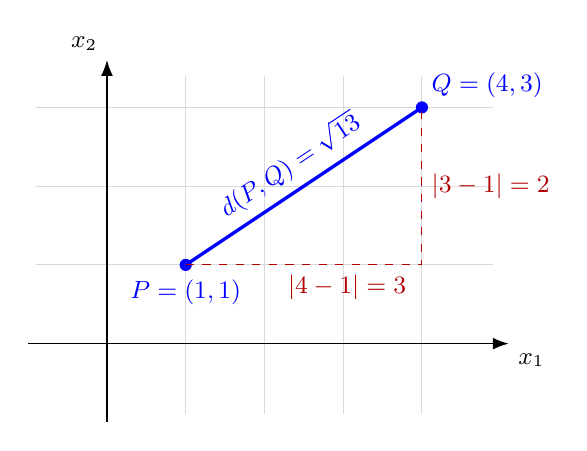
\begin{tikzpicture}[every node/.style={font=\small}, >={Latex[length=2mm]}]
	\draw[gray!30, step=1] (-0.9,-0.9) grid (4.9,3.4);
	\draw[->] (-1,0) -- (5.1,0) node[below right] {$x_1$};
	\draw[->] (0,-1) -- (0,3.6) node[above left] {$x_2$};
	\fill[blue] (1,1) circle (2.2pt) node[below, yshift=-2pt] {$P=(1,1)$};
	\fill[blue] (4,3) circle (2.2pt) node[above right] {$Q=(4,3)$};
	\draw[blue, very thick] (1,1) -- (4,3) node[midway, above, sloped] {$d(P,Q)=\sqrt{13}$};
	\draw[dashed, red!70!black] (1,1) -- (4,1) -- (4,3);
	\node[red!70!black, below] at (3.05,1) {$|4-1|=3$};
	\node[red!70!black, right, font=\small] at (4,2) {$|3-1|=2$};
\end{tikzpicture}
\end{document}
